\documentclass[tikz,border=10pt]{standalone}
% No extra packages or libraries needed for this figure.
\begin{document}
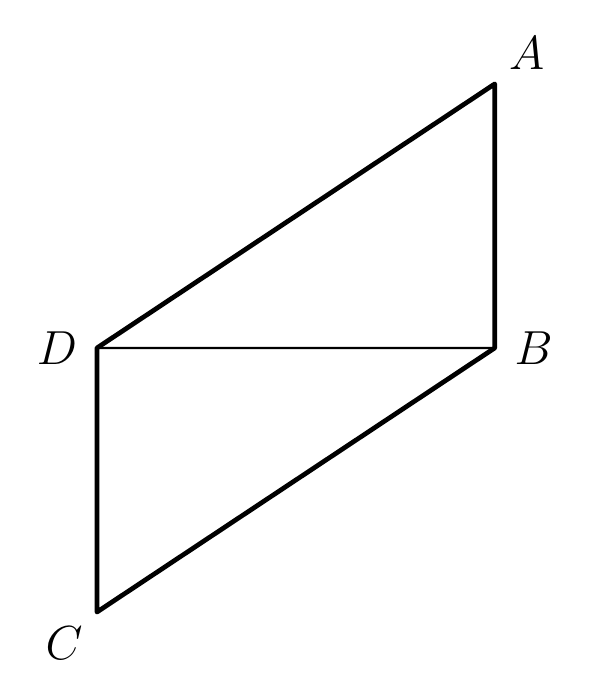
\begin{tikzpicture}[line width=1.7pt, line join=round]
  % Vertices (pixel -> cm, s = 0.02139, centred on ink bbox)
  \coordinate (A) at (2.5369452862893866,3.3695000634558463);
  \coordinate (B) at (2.5370546294706076,0.016082365775463382);
  \coordinate (C) at (-2.5149452862893864,-3.3375000634558463);
  \coordinate (D) at (-2.5150546294706073,0.015917634224536615);

  % Parallelogram sides (solid, black)
  \draw[solid, black] (A) -- (B) -- (C) -- (D) -- cycle;

  % Thin horizontal diagonal D to B
  \draw[solid, black, line width=0.8pt] (D) -- (B);

  % Labels in serif (Computer Modern), placed outside each vertex
  \node[above right=1pt] at (A) {\fontsize{17.5}{21}\selectfont $A$};
  \node[right=3pt] at (B) {\fontsize{17.5}{21}\selectfont $B$};
  \node[below left=1pt] at (C) {\fontsize{17.5}{21}\selectfont $C$};
  \node[left=3pt] at (D) {\fontsize{17.5}{21}\selectfont $D$};
\end{tikzpicture}
\end{document}